%%
%% This is file `sample-manuscript.tex',
%% generated with the docstrip utility.
%%
%% The original source files were:
%%
%% samples.dtx  (with options: `manuscript')
%% 
%% IMPORTANT NOTICE:
%% 
%% For the copyright see the source file.
%% 
%% Any modified versions of this file must be renamed
%% with new filenames distinct from sample-manuscript.tex.
%% 
%% For distribution of the original source see the terms
%% for copying and modification in the file samples.dtx.
%% 
%% This generated file may be distributed as long as the
%% original source files, as listed above, are part of the
%% same distribution. (The sources need not necessarily be
%% in the same archive or directory.)
%%
%% The first command in your LaTeX source must be the \documentclass command.
%%%% Small single column format, used for CIE, CSUR, DTRAP, JACM, JDIQ, JEA, JERIC, JETC, PACMCGIT, TAAS, TACCESS, TACO, TALG, TALLIP (formerly TALIP), TCPS, TDSCI, TEAC, TECS, TELO, THRI, TIIS, TIOT, TISSEC, TIST, TKDD, TMIS, TOCE, TOCHI, TOCL, TOCS, TOCT, TODAES, TODS, TOIS, TOIT, TOMACS, TOMM (formerly TOMCCAP), TOMPECS, TOMS, TOPC, TOPLAS, TOPS, TOS, TOSEM, TOSN, TQC, TRETS, TSAS, TSC, TSLP, TWEB.
% \documentclass[acmsmall]{acmart}

%%%% Large single column format, used for IMWUT, JOCCH, PACMPL, POMACS, TAP, PACMHCI
% \documentclass[acmlarge,screen]{acmart}

%%%% Large double column format, used for TOG
% \documentclass[acmtog, authorversion]{acmart}

%%%% Generic manuscript mode, required for submission
%%%% and peer review
\documentclass[manuscript,screen,review]{acmart}

\usepackage{todonotes}

%% Fonts used in the template cannot be substituted; margin 
%% adjustments are not allowed.
%%
%% \BibTeX command to typeset BibTeX logo in the docs
\AtBeginDocument{%
  \providecommand\BibTeX{{%
    \normalfont B\kern-0.5em{\scshape i\kern-0.25em b}\kern-0.8em\TeX}}}

%% Rights management information.  This information is sent to you
%% when you complete the rights form.  These commands have SAMPLE
%% values in them; it is your responsibility as an author to replace
%% the commands and values with those provided to you when you
%% complete the rights form.
\setcopyright{acmcopyright}
\copyrightyear{2018}
\acmYear{2018}
\acmDOI{10.1145/1122445.1122456}

%% These commands are for a PROCEEDINGS abstract or paper.
\acmConference[Woodstock '18]{Woodstock '18: ACM Symposium on Neural
  Gaze Detection}{June 03--05, 2018}{Woodstock, NY}
\acmBooktitle{Woodstock '18: ACM Symposium on Neural Gaze Detection,
  June 03--05, 2018, Woodstock, NY}
\acmPrice{15.00}
\acmISBN{978-1-4503-XXXX-X/18/06}


%%
%% Submission ID.
%% Use this when submitting an article to a sponsored event. You'll
%% receive a unique submission ID from the organizers
%% of the event, and this ID should be used as the parameter to this command.
%%\acmSubmissionID{123-A56-BU3}

%%
%% The majority of ACM publications use numbered citations and
%% references.  The command \citestyle{authoryear} switches to the
%% "author year" style.
%%
%% If you are preparing content for an event
%% sponsored by ACM SIGGRAPH, you must use the "author year" style of
%% citations and references.
%% Uncommenting
%% the next command will enable that style.
%%\citestyle{acmauthoryear}

%%
%% end of the preamble, start of the body of the document source.
\begin{document}

%%
%% The "title" command has an optional parameter,
%% allowing the author to define a "short title" to be used in page headers.
\title{Preserving Agency during Accelerated Human Action using Brain Signals reflecting Interaction Intent}
% Using Brain Signals of Interaction Intent to Trigger Accelerated Human Action preserves Agency

% Preconscious Interaction: Stimulating Muscles by Brain Signals of the Intent to Interact}

%%
%% The "author" command and its associated commands are used to define
%% the authors and their affiliations.
%% Of note is the shared affiliation of the first two authors, and the
%% "authornote" and "authornotemark" commands
%% used to denote shared contribution to the research.
\author{Lukas Gehrke}
% \authornote{Both authors contributed equally to this research.}
\email{lukas-gehrke@tu-berlin.de}
\orcid{1234-5678-9012}
\affiliation{%
  \institution{TU Berlin}
  \streetaddress{Straße des 17. Juni 135}
  \city{Berlin}
  \state{Berlin}
  \country{Germany}
  \postcode{10623}
}

%%
%% By default, the full list of authors will be used in the page
%% headers. Often, this list is too long, and will overlap
%% other information printed in the page headers. This command allows
%% the author to define a more concise list
%% of authors' names for this purpose.
\renewcommand{\shortauthors}{Gehrke et al.}

%%
%% The abstract is a short summary of the work to be presented in the
%% article.
\begin{abstract}
  
% Besides the title, this is what most people (90+%) will read from your paper!

% - [ ] Therefore, improve SEO (Search engine optimization): copy the abstract text to hemingwayapp.com to improve information density, keyword frequency and readability! Go through each sentence to shorten it and remove unnecessary words.

abstract text there only

\listoftodos
\end{abstract}

%%
%% The code below is generated by the tool at http://dl.acm.org/ccs.cfm.
%% Please copy and paste the code instead of the example below.
%%
\begin{CCSXML}
<ccs2012>
 <concept>
  <concept_id>10010520.10010553.10010562</concept_id>
  <concept_desc>Computer systems organization~Embedded systems</concept_desc>
  <concept_significance>500</concept_significance>
 </concept>
 <concept>
  <concept_id>10010520.10010575.10010755</concept_id>
  <concept_desc>Computer systems organization~Redundancy</concept_desc>
  <concept_significance>300</concept_significance>
 </concept>
 <concept>
  <concept_id>10010520.10010553.10010554</concept_id>
  <concept_desc>Computer systems organization~Robotics</concept_desc>
  <concept_significance>100</concept_significance>
 </concept>
 <concept>
  <concept_id>10003033.10003083.10003095</concept_id>
  <concept_desc>Networks~Network reliability</concept_desc>
  <concept_significance>100</concept_significance>
 </concept>
</ccs2012>
\end{CCSXML}

\ccsdesc[500]{Computer systems organization~Embedded systems}
\ccsdesc[300]{Computer systems organization~Redundancy}
\ccsdesc{Computer systems organization~Robotics}
\ccsdesc[100]{Networks~Network reliability}

%%
%% Keywords. The author(s) should pick words that accurately describe
%% the work being presented. Separate the keywords with commas.
\keywords{datasets, neural networks, gaze detection, text tagging}

%% A "teaser" image appears between the author and affiliation
%% information and the body of the document, and typically spans the
%% page.

% This is what most people (90+%) will see from your paper!

% - [ ]  use hemingwayapp.com (+SEO if hardcore) to make figure captions super precise
% - [ ]  are all the axes labels readable, font size 10 or up
% - [ ]  check for missing information: give someone the figure with captions to someone neutral to check if everything is clear from the figure alone
% - [ ]  for digital version: what is alt-text of figure, i.e. when hovering with the mouse over the figure what text appears next to the cursor
% - [ ]  for accessibility: write figure caption for the blind
%     - [ ]  explain what the figure shows
%     - [ ]  refactor using hemingwayapp.com

\begin{teaserfigure}
  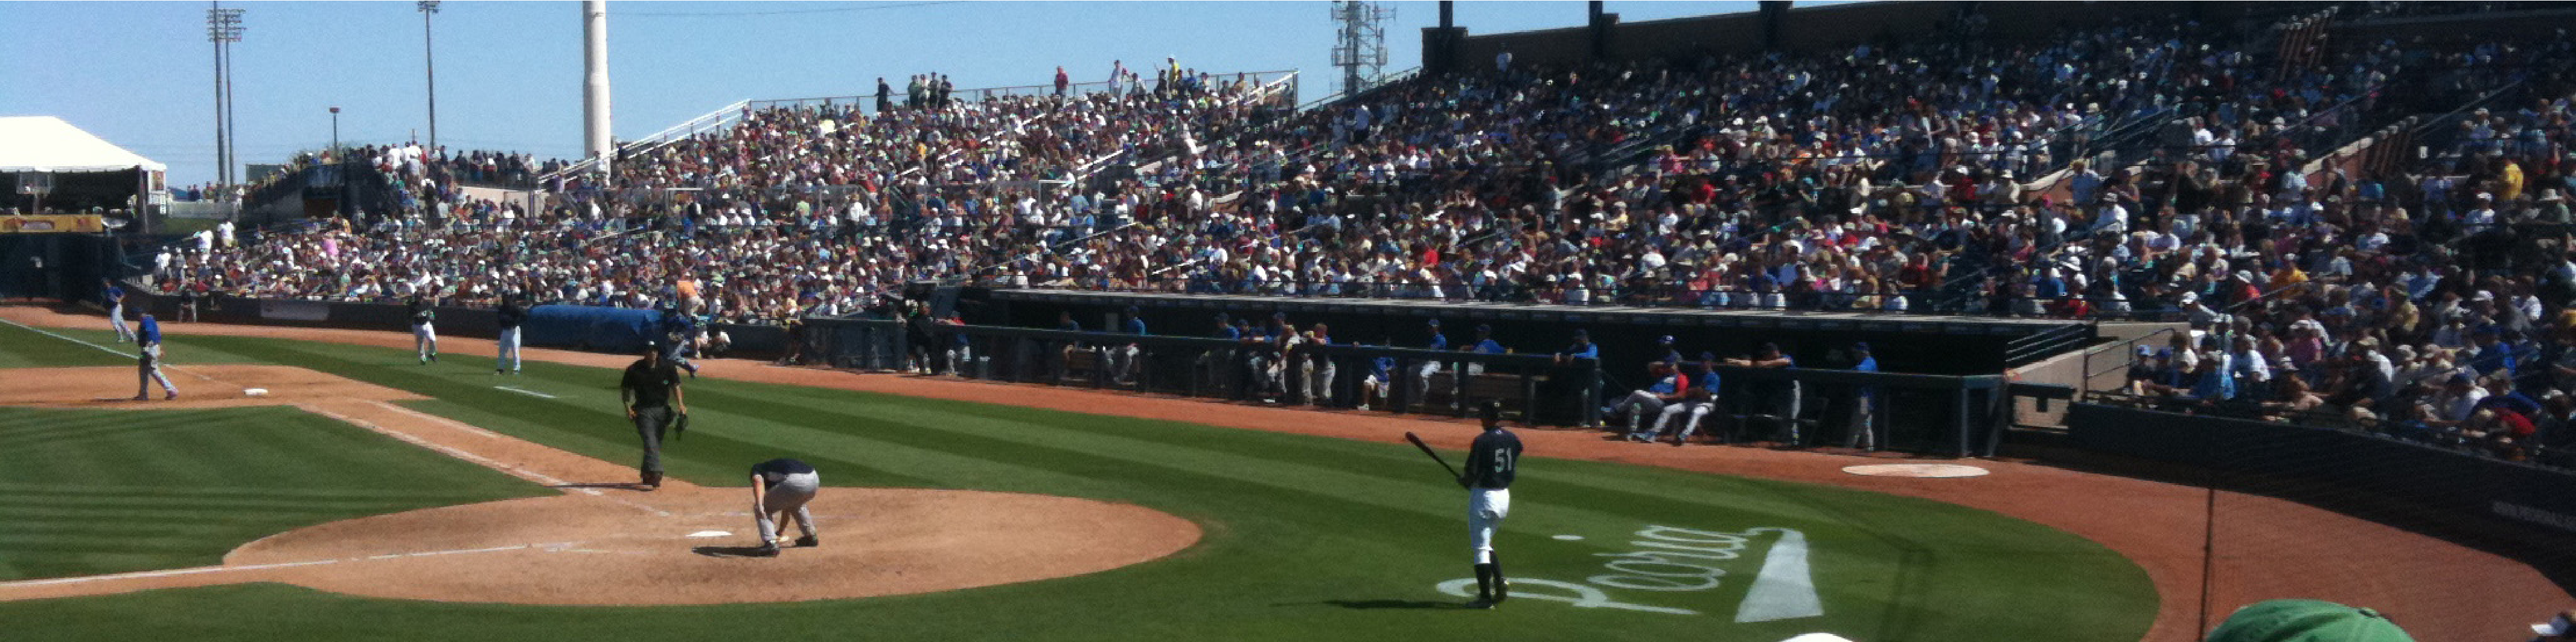
\includegraphics[width=\textwidth]{tex_sample_files/sampleteaser.pdf}
  \caption{Seattle Mariners at Spring Training, 2010.}
  \Description{Enjoying the baseball game from the third-base
  seats. Ichiro Suzuki preparing to bat.}
  \label{fig:teaser}
\end{teaserfigure}

%%
%% This command processes the author and affiliation and title
%% information and builds the first part of the formatted document.
\maketitle

\section{Introduction}
% 1. Describe the Current Situtation
% Functions as a starting point and a common basis. Therefore it primarily contains recognizable and agreed points.
% 2. What is the complication, challenge identified
% Spells the reason for acting now. It contains threats / opportunities and the hurdles that need to be overcome.
Technological advances in hardware that augment a user's physical actions have reignited dreams of overcoming human limitations, recovering lost abilities as well as simplifying skill acquisition. Wearable exoskeletons move a user's body by applying forces to the extremities, for example by pulling on the fingertips (see Dexmo Haptic Glove \footnote{https://www.dextarobotics.com/}) while electrical muscle stimulation (EMS) makes the user's extremities move by sending current into the muscle activating nerves. These technologies are becoming increasingly seamless to use. However, augmented user's frequently report dissociative experiences during or following augmented action. They do not experience agency.

The sense of agency refers to the experience of being in control of our own voluntary actions, instead of them feeling as though they randomly happen to us. This being in the "driving seat when it comes to our own actions"~\cite{Moore2016-ub} can be subdivided into the \textit{feeling} of agency, a low level pre-reflective sensory process, and a more higher level reflective cognitive process, the \textit{judgement} of agency~\cite{Moore2016-ub, Danry2022-xk}. The key challenge in human \textit{physical augmentation} is to create an experience of pre-reflective agency, so user's feel as though they are in the "driving seat" once again.
% if something happens for you in an interaction there is a cost to that:
% - impacts sense of agency which in turn makes user's engage less
% - impacts precision and accuracy, which can be very critical in high stakes scenarios, e.g. air traffic control

% 3. Question
% Asks the question how the hurdles of the Complication can be overcome. How can we prevent the threat or seize the opportunity? Also, what would be the benefits if the complication would be overcome?
% What have others done to address this and what do we propose "instead"
In physical augmentation, this experience of agency positively impacts performance.~\citet{Kasahara2019-sk} have shown that reaction times when tapping targets on a touchscreen can be increased by augmenting the user. Critically they found an optimal increase in reaction time, \textit{pre-emptive} gain, that preserves agency. At around 80 ms preceding the naturally occurring action, user's integrate the augmentation and maintain an experience of agency. However, setting this gain factor is dependent on each specific task and requires fitting the parameters over and over again. A key question remains: How can we maintain agency during physical augmentation without training and over-fitting parameters? In other words, how can we create closed systems for users to experience \textit{natural} augmentation?

% 4. (short) Answer Teaser
% Provides the answer on how to overcome the hurdles. Explains how this will help deflect the threats or seize the opportunities.
% keep this short
In this paper, we present a system that establishes a fast communication channel between the user's brain signals and a physical end effector, here EMS. The system controls the user's muscles through EMS at the time of the user's intent to act, as measured through readiness potentials (RP) present in the user's electroencephalogram (EEG). In our user study we then applied a mixed-methods research approach to investigate whether keeping the physical impact on the user's body in line with their intention to move, preserves their sense of agency.

\subsection{Preserving Agency using Brain Signals of the Intent to (Inter)act}
% 4. (long) Anwser with teaser image
% Provides the answer on how to overcome the hurdles. Explains how this will help deflect the threats or seize the opportunities.

%- not only physical integration but also other adpative interfaces, or control of mobile phone
\missingfigure{maybe small infographic here showing the connection from EEG volitional RP thought to EMS trigger on the Arm. <- better use this for the teaser image. Here better present the main results, i.e. sense of agency scores?}

% This is what most people (90+%) will see from your paper!

% - [ ]  use hemingwayapp.com (+SEO if hardcore) to make figure captions super precise
% - [ ]  are all the axes labels readable, font size 10 or up
% - [ ]  check for missing information: give someone the figure with captions to someone neutral to check if everything is clear from the figure alone
% - [ ]  for digital version: what is alt-text of figure, i.e. when hovering with the mouse over the figure what text appears next to the cursor
% - [ ]  for accessibility: write figure caption for the blind
%     - [ ]  explain what the figure shows
%     - [ ]  refactor using hemingwayapp.com

\begin{teaserfigure}
  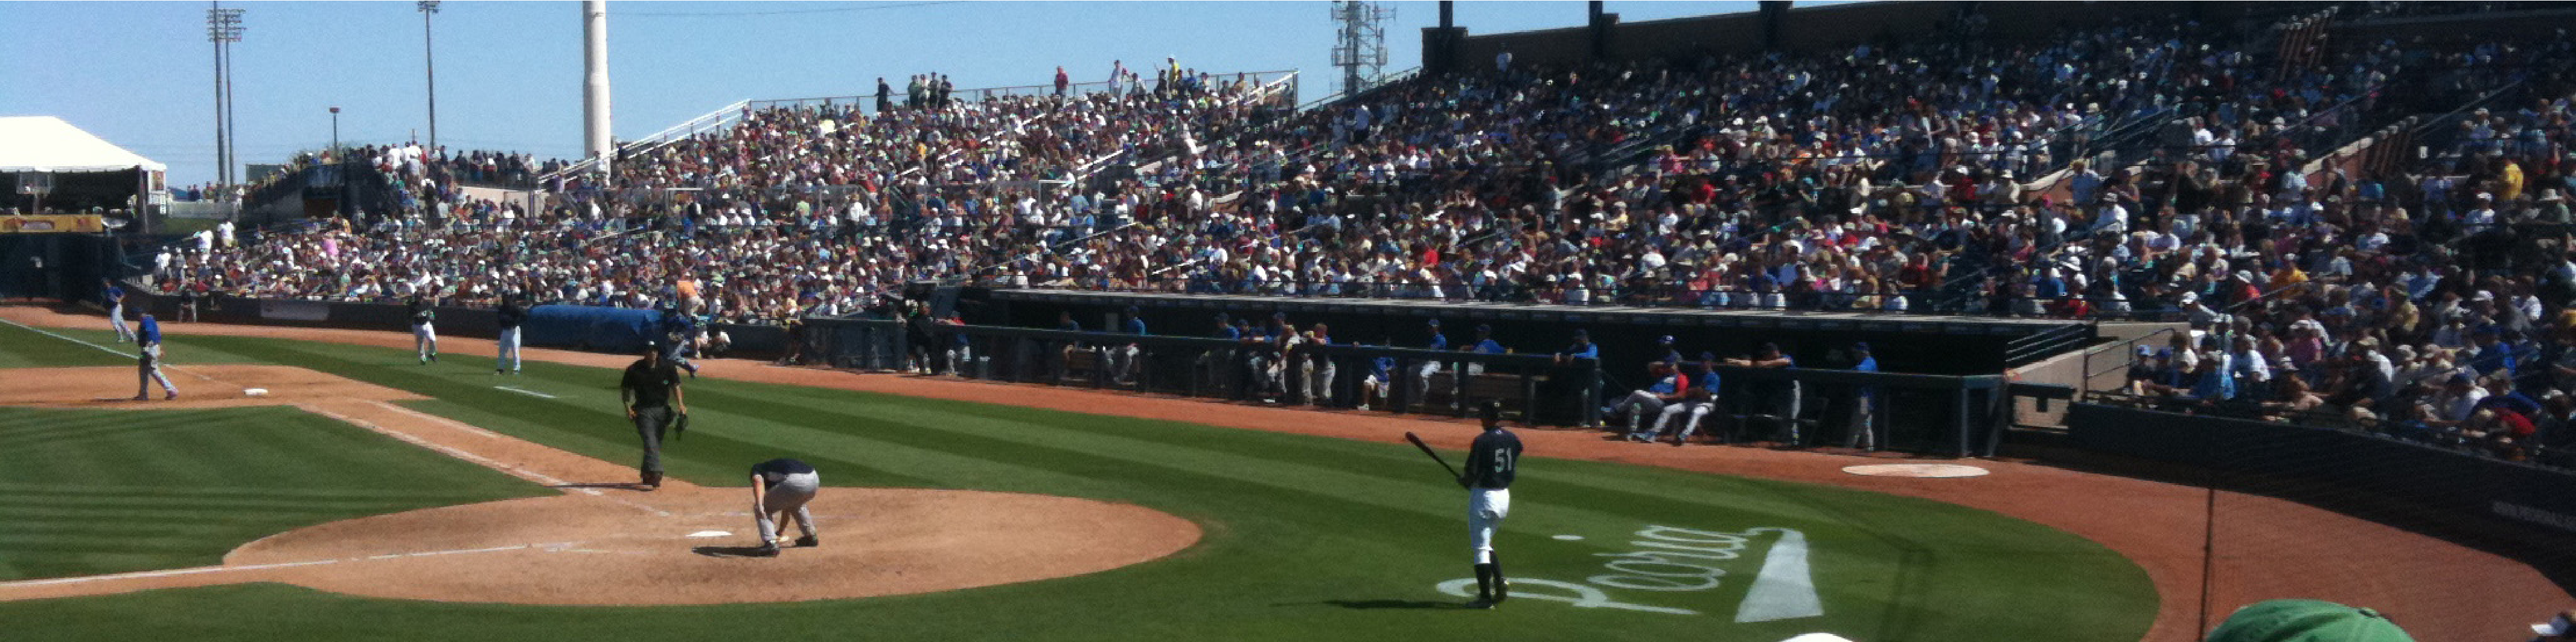
\includegraphics[width=\textwidth]{tex_sample_files/sampleteaser.pdf}
  \caption{Seattle Mariners at Spring Training, 2010.}
  \Description{Enjoying the baseball game from the third-base
  seats. Ichiro Suzuki preparing to bat.}
  \label{fig:teaser}
\end{teaserfigure}
\section{Related Work}
Our research draws inspiration from neuroscience and from engineering work on BCIs as well as on physical user augmentation. In order to situate our findings, we briefly review the literature on SoA specifically focusing on what it means to act at one's own volition, being a passive observer, and when acting integrated with a technology.

\subsection{Theories on Sense of Agency}
The most widely used theory on how the SoA arises is the \textit{comparator model}~\cite{Blakemore2002-dj, Frith2000-ch, Frith2006-sc}: When we act at our own volition and intentionally perform an action, the brain generates sensory predictions about the action outcome. These predictions are constantly compared to the actual sensory data available during the execution of the action. These include continuous signals such as proprioceptive and visual monitoring of the ongoing movement as well as higher level predictions about the semantic outcome of the action~\cite{Clark2013-ah, Haggard2003-ff, Haggard2017-uv}. If no sensorimotor incongruency arises, and further, the brain attributes subjective causality over the action outcome, SoA manifests. 

In the simple case of pressing a key on a piano, the finger movement is constantly compared to the predicted proprioceptive feedback. Subsequently, the tone generated by the key press is evaluated against auditory predictions. On a semantic level, these predictions may be in reference to whether the tone loudness corresponds to the velocity of the key press or whether the tone is in-key or out-of-key, and in general aligns with the subjective goal of the keypress~\cite{Pangratz2023-ew}. If these predictions -- based on the intended movement and its expected outcome -- explain the sensory data available, agency is experienced.
%, see figure~\ref{fig:task_design} INTENTION).

In human-computer interaction (HCI), these constructs are often categorized in slightly different terms. \textit{Pre-reflective} is used to describe `early', implicit, experience of agency, such as when matching proprioceptive predictions about finger movements. At higher levels of the cognitive hierarchy, \textit{reflective}, i.e. conscious, experience refers to matching semantic predictions about action outcomes~\cite{Danry2022-xk, Cornelio2022-aq}. 

In order to measure SoA, both explicit and implicit methods have been developed. Explicit methods directly query participants to report their subjective experiences using questionnaires. Items such as ``It felt like I was in control of the hand I was looking at''~\cite{Haggard2002-sz} or ``Indicate how much it felt like moving the joystick caused the object on the computer screen to move''~\cite{Ebert2010-lu}, query either the \textit{pre-reflective} action -- or the \textit{reflective} outcome evaluation~\cite{Moore2012-dk}. In most cases such questionnaires aim at a higher-level, reflective, judgment of agency.

On the other hand, implicit methods are often used to query low-level pre-reflective sensory predictions that are not consciously perceived~\cite{Moore2016-ub, Limerick2014-un, Moore2012-ic}. Seminal work in neuroscience has described one effect of SoA as a bias in the perception of action \textit{outcome}: Intentional binding paradigms state that when a button press is followed by a -- delayed -- outcome, e.g. a sound, participants mentally compress the delay~\cite{Haggard2002-sz}. In the theories original formulation, this temporal compression was assumed to only occur following movements that were intended: The action outcome is mentally \textit{bound} to the intention. To reduce uncertainty about the binding, the brain `explains away' the excess delta, compressing the action-outcome delay.

More recently it has been shown that this `temporal binding' also manifests when participants are merely a bystander witness in action-outcome scenarios~\cite{Suzuki2019-pi, Gutzeit2023-ei}. Among others, Suzuki et al.~\citep{Suzuki2019-pi} showed that temporal binding manifests as an effect of multisensory causal binding unrelated to intention or agency, e.g. binding effects were shown in scenarios where one is witnessing a replay of one's own earlier actions. Hence, it remains interesting to see how such binding manifests in \textit{integrated} user's.

% integration
As opposed to acting at one's own volition using one's own body, movement augmentation hardware allows moving a user's body even without their intention. Today, there are three main technologies to physically augment users' actions: Through the use of mechanical actuators, i.e., exoskeletons, a user's body can be moved by applying forces to the extremities~\cite{Kuhn2013-ls}. Another possibility is to stimulate the brain directly~\cite{Haggard2002-sz}, so the stimulation causes a motor response, for example by using transcranial magnetic stimulation (TMS). Lastly, electrical muscle stimulation (EMS) makes the user's extremities move by sending current into their muscle-activating nerves. Irrespective of the method applied, these technologies allow to move a user's body without the user having generated any predictions about the movement and its outcome. However, proprioceptive, visual, and other signals indicate that one's own body is moving. Hence, re-afference signals are present without an efference command and copy. Thus, concerning the comparator model, a prediction error will arise, negatively impacting SoA~\cite{Wen2020-dk}.

% none or a decreased SoA will be observed in the case of externally controlled actions, for example by brain stimulation or when the body is moved by another person~\cite{Kuhn2013-ls}. With something or somebody else moving our body to perform, e.g., a key press on a piano, the lack of intention to play the piano -- and derived sensory and semantic predictions -- negatively impacts the experience of agency.

% \subsubsection{Measuring Sense of Agency}
% Both explicit and implicit methods have been developed to evaluate the sense of agency. These methods provide the basis to investigate the effects of action augmentation technology on agency experience. 

% Explicit methods directly query participants to report their subjective experiences using questionnaires. Items such as ``It felt like I was in control of the hand I was looking at''~\cite{Haggard2002-sz} or ``Indicate how much it felt like moving the joystick caused the object on the computer screen to move''~\cite{Ebert2010-lu}, query either the \textit{pre-reflective} action -- or the \textit{reflective} outcome evaluation~\cite{Moore2012-dk}. In most cases such questionnaires aim at a higher-level, reflective, judgment of agency. 

% On the other hand, implicit methods are often used to query low-level pre-reflective sensory predictions that are not consciously perceived~\cite{Moore2016-ub, Limerick2014-un, Moore2012-ic}. Seminal work in neuroscience has described one effect of SoA as a bias in the perception of action \textit{outcome}: Intentional binding paradigms state that when a button press is followed by a -- delayed -- outcome, participants mentally compress the delay~\cite{Haggard2002-sz}. In the theories original formulation, this temporal compression was assumed to only occur following movements that were intended: The action outcome is mentally \textit{bound} to the intention. To reduce uncertainty about the binding, the brain `explains away' the excess delta, compressing the action-outcome delay~\cite{Barlas2018-bq}. 

% % introduce temporal binding -- intentional binding as a measure frequently used in neuroscience and what is the state-of-the-art of the separation of these phenomena
% % ~\cite{Wen2020-dk} - prediction errors


% Supplementing this behavioral phenomenon, physiological evidence can prove useful to further understand the interplay between volitional action and the SoA.

\subsection{Controlling Actuated Haptic Experiences}

Experimental setups to investigate new `on-body' augmentation technologies that aim to preserve the user's SoA, frequently use highly controlled `stimulus-response' paradigms. For example, scenarios where participants are instructed to tap on a touchscreen in response to a presented stimulus on the screen. Here, participants' behavior can be predicted with very high certainty to follow the presented stimulus, and estimating their reaction time is very accurate. In such controlled scenarios, the timing of an action augmentation device can be tuned to be near optimal. Hence, \textit{pre-empting} the user's motion can be designed to fall in line with their intention to move, thereby maintaining SoA. Previously, ~\citet{Kasahara2019-sk} used a reaction time task in which participants had to tap a target on screen as soon as it appeared and subsequently rate their SoA. They showed that in such a scenario, user's actions can be pre-empted and that a pre-emption of about 80 ms best preserves agency~\cite{Kasahara2019-sk, Kasahara2021-gy}. 

This is in line with evidence from cognitive neuroscience which indicates that from around 200 ms before a voluntary movement, users are unable to ``veto'' their self-initiated movement~\cite{Schultze-Kraft2016-bx}. After this ``point of no return'' user's struggle to assign a source other than themselves to the action initiation. Here, the \textit{key} aspect for SoA in action augmentation becomes apparent: External influences on the user's body need to be in line with the user's intention to act. Crucially then, a key challenge remaining is to design systems that maintain agency when user's actions are unpredictable and where the experimenter does \textit{not} have executive control over the environment. In other words, how can a closed-loop system to deliver a \textit{natural} agency experience for users' augmented actions be designed?

\subsubsection{Using Brain Signals Reflecting the Intent to (Inter-)act for Action Augmentation}
One possible design solution is to leverage physiological signals for action augmentation. Of the possible physiological signals that can be leveraged, the EEG is very well suited because of its high temporal resolution and the non-invasive recording close to the motor command generating structures in the human brain. 

The RP, or \textit{lateralized readiness potential}, is an amplitude fluctuation in the ongoing EEG activity that has frequently been observed preceding voluntary action~\cite{Deecke1969-bl, Libet1983-qu}. The RP is reliably observed at electrodes placed over the sensorimotor cortex contralateral to the acting hand. In the extended 10-20 system for EEG electrode placement~\cite{Jasper1983-uw}, these are electrodes C3 located over the sensorimotor cortex of the left hemisphere, and C4 vice versa. However, activity observed at electrode Cz is reported most frequently as it reflects neural activity originating from the sensorimotor cortex without lateralization bias. Since the RPs' measurable onset precedes the time of participants' self-reported conscious movement intention, it has drawn much interest with respect to the debate on free will, see~\cite{Schurger2021-vp} for a recent neuroscientific perspective. However, evidence abounds for its role in action preparation. An RP is typically comprised of two stages: an early slow stage that begins up to two seconds before the actual movement and a late steep stage that starts about 400 milliseconds before movement. The first stage manifests in the pre-supplementary motor area and transfers to the premotor cortex shortly after. The second stage manifests contra-laterally in the primary motor cortex~\cite{Shibasaki2006-mt}. 

A recent study has shown that the RP is ingrained in the subconscious mechanisms preceding movements that people cannot explicitly suppress~\cite{Schultze-Kraft2021-cu}. In their study,~\citet{Schultze-Kraft2021-cu} asked participants to find a way to perform voluntary movements while keeping accompanying RP amplitudes as small as possible. After each trial they informed participants about the strength of the RP in the current trial, so participants had a feedback metric to optimize for. They found participants unable to suppress their RP. This inability to suppress the RP renders it a reliable feature for classification. For example, the RP can be detected in real-time using a brain-computer interface (BCI).~\citet{Schultze-Kraft2016-bx} demonstrated a prototype that detects RPs in participants ongoing EEG data and adapts an interface accordingly. In their study, participants were instructed to veto their self-initiated movement whenever a red dot occurred on the screen. The red dot's appearance was controlled by the BCI. Whenever an RP was detected, the red dot appeared. The authors found that participants were able to veto their self-initiated movement if the red dot appeared no later than 200ms preceding their movement onset. After that, participants were unable to ``overwrite'' their motor command and acted regardless of the red dot's appearance on screen.

Taken together, these findings demonstrated that the RP is a reliable signal preceding voluntary movement initiation and hence, is a well-suited candidate to base (neuro)--adaptive systems on.


% Gender-inclusive: Relevant throughout the document but frequently occuring here:
% - [ ]  write gender-inclusive: do not use he or she but use they instead: "the participant was asking..., he liked ... → they liked (in singular)
% check for the following:
% - [ ]  Have you used “man” or “men” or words containing them to refer to people who may not be men?
% - [ ]  Have you used “he,” “him,” “his,” or “himself” to refer to people who may not be men?
% - [ ]  If you have mentioned someone’s sex or gender, was it necessary to do so?
% - [ ]  Do you use any occupational (or other) stereotypes?
% - [ ]  Do you provide the same kinds of information and descriptions when writing about people of different genders?

\section{User Study}

\section{Methods}
\section{Results}

\subsection{Human-Computer Collaboration for Human Augmentation}
\missingfigure{A: Boxplot of questionnaire scores, are they significantly better than 0? Are they significantly better then after the training? -> frame the training the same as the experiment, B: Sentiment Word Clouds}

% system usability score

% sentiment analysis ttest the counts?

% Did they get faster? Calculate time between hand motion onset and button press. If yes, evidence that there was acceptance for the help/augmentation the system provided

\subsection{The BCI}

\missingfigure{!: grand average ERP at Cz comparing idle vs. movement intention with scalp map of voltage across all channels in the last [-100 0] interval of both idle and pre-move; B: What did the windows mean features look like. Boxplot with idle vs. pre-move and single observations}

% ttest of amplitudes in last time window

% classification accuracy

\missingfigure{confusion matrix!, AUC, ROC -> in discussion mention that we want to do that continuously and not only look at the times preceding hand movement but at all time points}
\section{Discussion}

% summary here! BLUF!

% Strength of EMS could be set by the amplitude of the RP -> is there evidence for a correlation between amplitude and 'strength' of volitional action?

% EEG Signal heavily contaminated by eye movement, maybe a worthwhile thing to build this interaction relying solely on eye tracking information, gaze fixating on the target before moving
\section{Conclusions, Limitations and Opportunities}

%%
%% The acknowledgments section is defined using the "acks" environment
%% (and NOT an unnumbered section). This ensures the proper
%% identification of the section in the article metadata, and the
%% consistent spelling of the heading.
\begin{acks}

% no section, just write down the acknowledgements as text
\end{acks}

%%
%% The next two lines define the bibliography style to be used, and
%% the bibliography file.
\bibliographystyle{ACM-Reference-Format}
\bibliography{input/paperpile}

%%
%% If your work has an appendix, this is the place to put it.
\appendix


% appendix sections if necessary

\end{document}
\endinput
%%
%% End of file `sample-authordraft.tex'.
